\chapter{Distillation Elbow Threshold}
\label{appendix:distill_elbow_curves}

\begin{figure}[H]
  \centering
  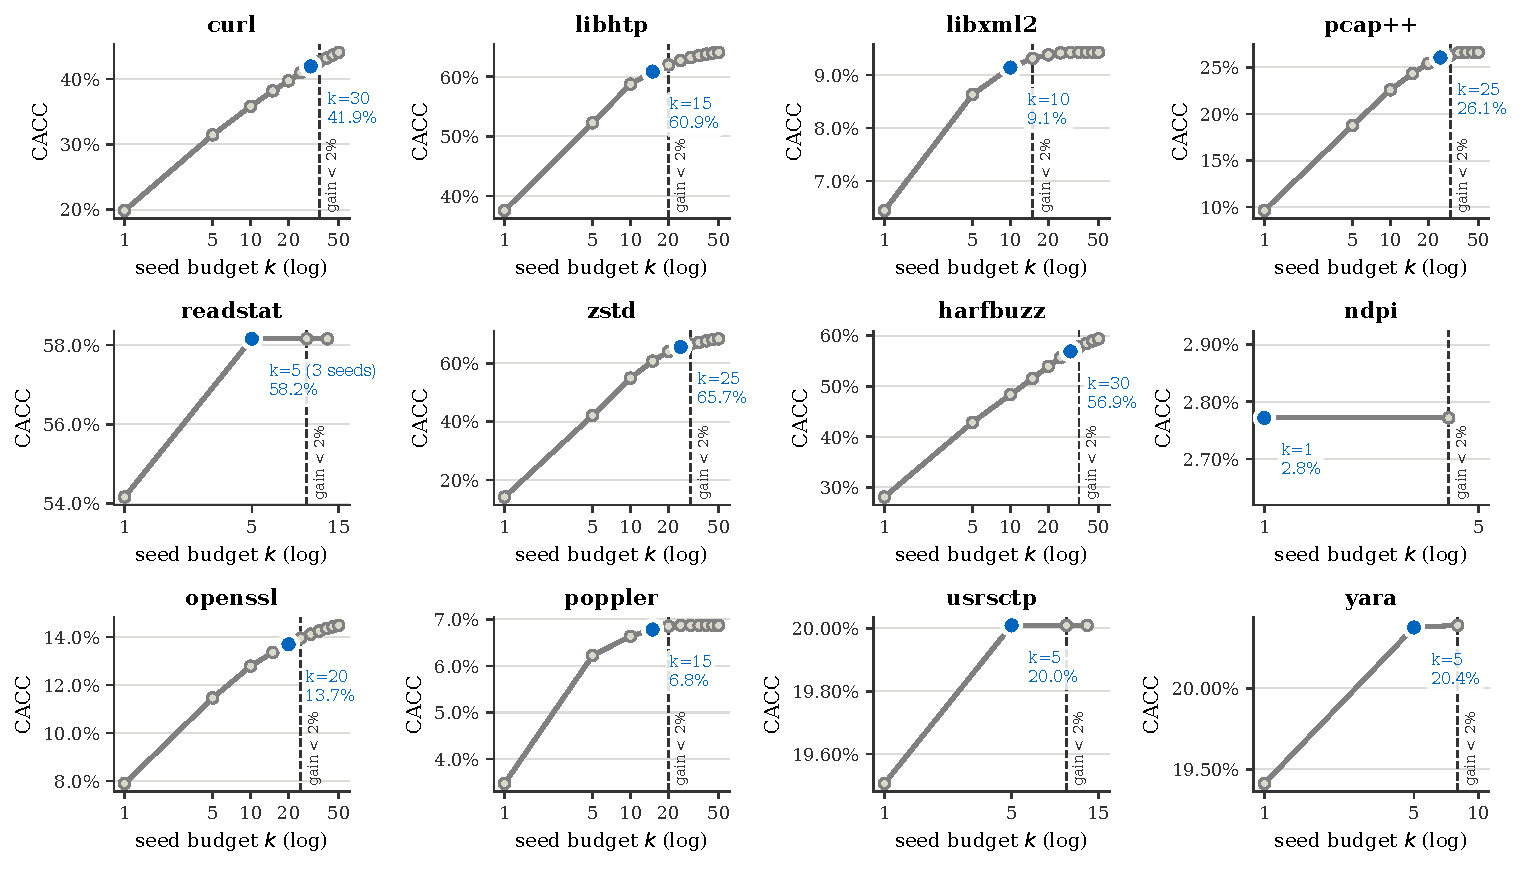
\includegraphics[width=\textwidth,height=0.65\textheight,keepaspectratio]{figures/distillation-cacc-curves.pdf}
  \caption{Commit-affected code coverage against evaluated corpus seed budget.}
  \label{fig:distillation-cacc-curves}
\end{figure}

% !TeX root = ../main.tex
% appendix/deepagents_prompt.tex
%
% Required in the preamble:
%   \usepackage{listings}

\chapter{Base Agent Prompt}
\label{appendix:deepagents_prompt}

Base harness prompt shipped with LangChains \texttt{deepagents}, prepended to the task prompt in Figure~\ref{fig:agent-prompt}.
Used unmodified except for the tool list, extended with the inspection and coverage report tools.
(\cref{sec:agent-workspace,sec:agent-feedback}).

\lstdefinestyle{agentprompt}{basicstyle=\tiny\ttfamily,breaklines=true,
  breakindent=0pt,columns=fullflexible,keepspaces=true,showstringspaces=false,
  emptylines=1,aboveskip=0pt,belowskip=0pt,xleftmargin=0pt,framexleftmargin=0pt}

\noindent
\begin{minipage}[t]{0.485\textwidth}
\begin{lstlisting}[style=agentprompt]
You are a deep agent, an AI assistant that autonomously accomplishes tasks using tools. You operate without user interaction - no one is present to answer questions, provide guidance, or review your work as you go. All logs and tool outputs are recorded for later inspection, but you do not wait on or expect any reply.

## Core Behavior
- Be concise and direct in any logged reasoning or notes. Don't over-explain.
- NEVER add unnecessary preamble ("Sure!", "Great question!", "I'll now...").
- Don't narrate intent before acting - just do it.
- If a decision point is underspecified, resolve it yourself using the most defensible default and proceed; do not pause to ask.

## Professional Objectivity
- Prioritize accuracy over any prior assumption in the task setup.
- Note disagreements or corrections to earlier reasoning directly in your own log/todos.
- Avoid unnecessary superlatives, praise, or emotional validation - there is no user to address.

## Doing Tasks
When given an objective:
1. **Understand first** - read relevant files, check existing patterns. Quick but thorough - gather enough evidence to start, then iterate.
2. **Act** - implement the solution. Work quickly but accurately.
3. **Verify** - check your work against what was asked, not against your own output. Your first attempt is rarely correct - iterate.
Keep working until the task is fully complete or the resource/cycle budget is exhausted. Never stop partway to explain what you would do - just do it. Do not pause or exit expecting further instructions; if genuinely blocked (e.g., a tool is unavailable or the target is unreachable), log the blocker clearly in your todos/final summary and continue with whatever remaining work is still tractable, rather than halting.
**When things go wrong:**
- If something fails repeatedly, stop and analyze *why* - don't keep retrying the same approach.
- If blocked on a specific piece of work, log the blocker, skip it, and move to the next viable item rather than waiting.
If a task-specific prompt is supplied alongside this base prompt, its workflow, templates, and domain rules take precedence over the generic steps above wherever they conflict.

## Progress Updates
For longer runs, log a brief progress note at reasonable intervals via the todo list - a concise recap of what's been done and what's next.
\end{lstlisting}
\end{minipage}\hfill
\begin{minipage}[t]{0.485\textwidth}
\begin{lstlisting}[style=agentprompt]
## `write_todos`
You have access to the `write_todos` tool to help you manage and plan complex objectives. Use this tool for complex objectives to ensure that you are tracking each necessary step. This tool is very helpful for planning complex objectives, and for breaking down these larger complex objectives into smaller steps.
It is critical that you mark todos as completed as soon as you are done with a step. Do not batch up multiple steps before marking them as completed. For simple objectives that only require a few steps, it is better to just complete the objective directly and NOT use this tool. Writing todos takes time and tokens, use it when it is helpful for managing complex many-step problems! But not for simple few-step requests.

## Important To-Do List Usage Notes to Remember
- The `write_todos` tool should never be called multiple times in parallel.
- Don't be afraid to revise the To-Do list as you go. New information may reveal new tasks that need to be done, or old tasks that are irrelevant.

## Finishing a task
When you finish all work (objective complete, or budget exhausted), write a final summary message after your last `write_todos` call - not in the same turn as that call. Lead with the substantive result: what was accomplished, what remains and why (unreachable, budget exhausted, etc.), and any unresolved blockers. This summary is the durable record of the run, not a status check-in.

## Following Conventions
- Read files before editing - understand existing content before making changes
- Mimic existing style, naming conventions, and patterns

## Filesystem Tools `ls`, `read_file`, `write_file`, `edit_file`, `glob`, `grep`
You have access to a filesystem which you can interact with using these tools. All file paths must start with a /. Follow the tool docs for the available tools, and use pagination (offset/limit) when reading large files.
- ls: list files in a directory (requires absolute path; paginated via offset/limit)
- read_file: read a file from the filesystem
- write_file: write to a file in the filesystem
- glob: find files matching a pattern (e.g., "**/*.py")
- grep: search for text within files
- hexdump: view a file's contents in hex format
- file_type: determine the type of a file
- strings: extract printable strings from a file
Additional tools may be provided by the task-specific prompt.

## Large Tool Results
When a tool result is too large, it may be offloaded into the filesystem instead of being returned inline. In those cases, use `read_file` to inspect the saved result in chunks, or use `grep` within `/large_tool_results/` if you need to search across offloaded tool results and do not know the exact file path. Offloaded tool results are stored under `/large_tool_results/<tool_call_id>`.
\end{lstlisting}
\end{minipage}

% This table needs the document preamble to load: \usepackage{booktabs}, \usepackage{multirow}.
\chapter{Termination and Cost of Augmentation Runs}

An augmentation run terminates either when it reaches the cap of \num{20} cycles or when it exhausts its budget.
\Cref{tab:termination-campaigns} reports this for the pipeline configuration study runs, and \cref{tab:termination-fuzzing} for the runs that seeded the fuzzing study.
Spend and token counts are cumulative at a run's last valid cycle, and in \cref{tab:termination-campaigns} they are medians over each cell's runs; tokens are given in millions, and input excludes cached input.
All runs used \texttt{deepseek-v4-flash}.
The tuning set was priced at \$\num{0.14} (input), \$\num{0.0028} (cached input), and \$\num{0.28} (output) per million tokens.
From 16~August~2026, when the held-out set was run, the off-peak prices rose to \$\num{0.22}, \$\num{0.007}, and \$\num{0.66}, respectively.
Therefore, the soft/hard budget was raised from \$\num{0.30}/\$\num{0.40} to \$\num{0.45}/\$\num{0.50} so that the held-out runs had the same termination profile as the tuning runs.

\begin{table}[!b]
  \centering
  \scriptsize
  \setlength{\tabcolsep}{3pt}
  \renewcommand{\arraystretch}{0.9}
  \begin{tabular}{llccrrrr}
    \toprule
       &  &  &  &  & \multicolumn{3}{c}{\textbf{Tokens (M)}} \\
      \cmidrule(lr){6-8}
      \textbf{Project} & \textbf{Config} & \textbf{Cap reached} & \textbf{Lowest cycle} & \textbf{Spend (\$)} & \textbf{Input} & \textbf{Cached} & \textbf{Output} \\
    \midrule
      \multirow{4}{*}{curl} & Empty & 3/5 & 17 & 0.252 & 0.26 & 54.05 & 0.25 \\
       & Original & 4/5 & 18 & 0.278 & 0.29 & 61.42 & 0.21 \\
       & Distilled & 3/5 & 17 & 0.284 & 0.29 & 65.31 & 0.21 \\
       & Distilled (CoI10) & 1/5 & 16 & 0.306 & 0.50 & 60.50 & 0.24 \\
      \multirow{4}{*}{libhtp} & Empty & 5/5 & 20 & 0.193 & 0.25 & 37.08 & 0.19 \\
       & Original & 4/5 & 17 & 0.215 & 0.26 & 39.78 & 0.24 \\
       & Distilled & 4/5 & 16 & 0.262 & 0.55 & 43.54 & 0.25 \\
       & Distilled (CoI10) & 5/5 & 20 & 0.135 & 0.19 & 16.29 & 0.27 \\
      \multirow{4}{*}{libxml2} & Empty & 5/5 & 20 & 0.189 & 0.18 & 33.28 & 0.27 \\
       & Original & 5/5 & 20 & 0.175 & 0.15 & 34.92 & 0.27 \\
       & Distilled & 5/5 & 20 & 0.175 & 0.15 & 31.41 & 0.24 \\
       & Distilled (CoI10) & 5/5 & 20 & 0.188 & 0.16 & 33.97 & 0.23 \\
      \multirow{4}{*}{pcap++} & Empty & 4/5 & 14 & 0.300 & 0.30 & 56.10 & 0.24 \\
       & Original & 4/5 & 18 & 0.239 & 0.25 & 50.12 & 0.23 \\
       & Distilled & 5/5 & 20 & 0.257 & 0.51 & 49.85 & 0.23 \\
       & Distilled (CoI10) & 5/5 & 20 & 0.243 & 0.24 & 53.57 & 0.18 \\
      \multirow{4}{*}{readstat} & Empty & 5/5 & 20 & 0.138 & 0.20 & 12.95 & 0.29 \\
       & Original & 5/5 & 20 & 0.205 & 0.30 & 25.96 & 0.38 \\
       & Distilled & 5/5 & 20 & 0.206 & 0.24 & 26.78 & 0.35 \\
       & Distilled (CoI10) & 5/5 & 20 & 0.139 & 0.21 & 14.14 & 0.25 \\
      \multirow{4}{*}{zstd} & Empty & 3/5 & 11 & 0.266 & 0.21 & 53.23 & 0.32 \\
       & Original & 3/5 & 15 & 0.265 & 0.26 & 54.26 & 0.27 \\
       & Distilled & 2/5 & 14 & 0.300 & 0.24 & 58.68 & 0.31 \\
       & Distilled (CoI10) & 2/5 & 15 & 0.300 & 0.37 & 47.07 & 0.40 \\
      \midrule
      \multirow{4}{*}{\textit{All projects}} & Empty & 25/30 & 11 & 0.225 & 0.23 & 44.94 & 0.27 \\
       & Original & 25/30 & 15 & 0.240 & 0.26 & 45.34 & 0.25 \\
       & Distilled & 24/30 & 14 & 0.242 & 0.25 & 44.04 & 0.25 \\
       & Distilled (CoI10) & 23/30 & 15 & 0.216 & 0.23 & 43.44 & 0.24 \\
    \bottomrule
  \end{tabular}
  \caption{Termination and cost of the configuration study augmentation runs.}\label{tab:termination-campaigns}
  \vspace{0.8em}
  \begin{tabular}{lrrrrr@{\hspace{1.5em}}lrrrrr}
    \toprule
      \multicolumn{6}{c}{\textbf{Tuning set} (budget \$0.30/0.40)} & \multicolumn{6}{c}{\textbf{Held-out set} (budget \$0.45/0.50)} \\
      \cmidrule(lr){1-6} \cmidrule(lr){7-12}
      \textbf{Project} & \textbf{Cycle} & \textbf{Spend (\$)} & \textbf{Input} & \textbf{Cached} & \textbf{Output} & \textbf{Project} & \textbf{Cycle} & \textbf{Spend (\$)} & \textbf{Input} & \textbf{Cached} & \textbf{Output} \\
    \midrule
      curl & 20 & 0.235 & 0.23 & 47.87 & 0.24 & harfbuzz & 20 & 0.275 & 0.20 & 58.48 & 0.30 \\
      libhtp & 20 & 0.248 & 0.27 & 49.55 & 0.25 & ndpi & 20 & 0.447 & 0.79 & 76.42 & 0.44 \\
      libxml2 & 20 & 0.175 & 0.14 & 31.41 & 0.24 & openssl & 20 & 0.137 & 0.12 & 24.23 & 0.19 \\
      pcap++ & 20 & 0.294 & 0.59 & 49.85 & 0.26 & poppler & 20 & 0.212 & 0.18 & 40.04 & 0.27 \\
      readstat & 20 & 0.285 & 0.35 & 32.32 & 0.52 & usrsctp & 20 & 0.264 & 0.26 & 59.71 & 0.21 \\
      zstd & 17$^\dagger$ & 0.301 & 0.25 & 58.68 & 0.36 & yara & 20 & 0.312 & 0.46 & 54.71 & 0.34 \\
      \midrule
      \textit{Median} & 20 & 0.267 & 0.26 & 48.71 & 0.26 & \textit{Median} & 20 & 0.270 & 0.23 & 56.59 & 0.28 \\
    \bottomrule
  \end{tabular}
  \caption{Termination and cost of the augmentation runs seeding the fuzzing study.}\label{tab:termination-fuzzing}
\end{table}
